% ============================================================
%  IEEE Conference Paper: The Paradigm Shift
%  Formatting: IEEEtran, two-column, 10 pt
%  Images: include the PNG files in the same directory as this .tex file
%  Small inline images are replaced with proper LaTeX math/symbols.
% ============================================================

\documentclass[conference]{IEEEtran}

% ---- Packages -----------------------------------------------
\usepackage[T1]{fontenc}
\usepackage[utf8]{inputenc}
\usepackage{amsmath,amssymb,amsfonts}
\usepackage{graphicx}
\usepackage{booktabs}        % professional table rules
\usepackage{array}
\usepackage{multirow}
\usepackage{url}
\usepackage{cite}
\usepackage{hyperref}
\usepackage{balance}         % balance last page columns
\usepackage[caption=false,font=footnotesize]{subfig}

% IEEEtran recommended hyperref settings
\hypersetup{colorlinks=false}

% ---- Custom math commands -----------------------------------
\newcommand{\Ltwonorm}[1]{\left\|#1\right\|_{2}}
\newcommand{\bigO}[1]{\mathcal{O}\!\left(#1\right)}

% =============================================================
\begin{document}

% ---- Title --------------------------------------------------
\title{The Paradigm Shift: From Model Scaling to Data-Centric Pipelines
       in Video Contextualization\\
       {\large An Ablation of Tokenization and Compression for Edge MLLMs}}

% ---- Authors ------------------------------------------------
\author{%
  \IEEEauthorblockN{Mian Afzal Saeed}
  \IEEEauthorblockA{Data Science Department\\
    FAST--National University of Computer\\
    and Emerging Sciences\\
    Lahore, Pakistan\\
    l232505@lhr.nu.edu.pk}
  \and
  \IEEEauthorblockN{Faryal Zahra}
  \IEEEauthorblockA{Data Science Department\\
    FAST--National University of Computer\\
    and Emerging Sciences\\
    Lahore, Pakistan\\
    l232551@lhr.nu.edu.pk}
  \and
  \IEEEauthorblockN{Hira Khalid}
  \IEEEauthorblockA{Data Science Department\\
    FAST--National University of Computer\\
    and Emerging Sciences\\
    Lahore, Pakistan\\
    l233594@lhr.nu.edu.pk}
}

\maketitle

% ---- Abstract -----------------------------------------------
\begin{abstract}
The deployment of Multimodal Large Language Models (MLLMs) for
spatial-temporal video understanding is severely constrained by the
memory bandwidth and compute limitations of edge hardware. Traditional
video preprocessing methods, such as aspect-ratio-preserving padding,
introduce ``dead'' visual tokens that aggressively bloat Key-Value (KV)
Cache allocation. When processing extended video sequences, this
computational waste frequently results in Out-Of-Memory (OOM) failures
on devices with limited VRAM\@. To address this bottleneck, we propose a
synthesized 5-Tier Temporal Compression Pipeline combined with a
``Naive Warping'' tokenization strategy designed to maximize token density.

We conduct a comprehensive ablation study using the Qwen2.5-VL
architecture (3B and 7B parameters) evaluated across the 20
spatial-temporal tasks of MVBench on heavily constrained hardware (Dual
Nvidia T4 GPUs). Our empirical results demonstrate that Naive Warping
achieves a near 50\% theoretical reduction in VRAM allocation without
degradation in zero-shot accuracy compared to standard padding methods.
Furthermore, we reveal an edge-scaling paradox where the 3B parameter
model statistically matches the 7B model in accuracy (52.11\% vs.\
51.68\% at $224{\times}224$) while sustaining significantly higher decode
throughput. Ultimately, we establish that heavily compressed, unpadded
visual tokenization paired with highly optimized, smaller-parameter
architectures forms the optimal configuration for real-time edge
deployment.

\textit{Note: The findings presented herein represent initial validation
results; further robust empirical testing is currently in progress to
achieve full production readiness.}
\end{abstract}

\begin{IEEEkeywords}
Edge AI, Multimodal Large Language Models, Video Understanding,
Tokenization, Visual Token Compression, KV Cache, Naive Warping,
Temporal Compression, Ablation Study
\end{IEEEkeywords}

% =============================================================
\section{Introduction}
\label{sec:intro}

As Multimodal Large Language Models (MLLMs) achieve state-of-the-art
performance in complex video understanding tasks, a problematic industry
paradigm has emerged: relying entirely on massive parameter scaling
(e.g., 70B+ models) to solve complex reasoning. This paradigm restricts
deployment to high-end cloud infrastructure. Edge environments---such as
autonomous robotics, local surveillance nodes, and drone navigation
systems---lack the massive VRAM capacity required to cache the dense
sequences of visual tokens generated by modern Vision Transformers
(ViTs).

Video data is inherently multidimensional; unlike a single static image,
a video stream multiplies the required token count by its temporal length
($T \times H \times W$). On constrained hardware, such as dual Nvidia T4
GPUs (15\,GB VRAM each), processing multi-frame high-resolution video
reliably induces memory bandwidth bottlenecks. Because the transformer's
self-attention mechanism scales quadratically $\bigO{N^2}$ with sequence
length, passing unoptimized video frames directly into an MLLM guarantees
rapid exhaustion of the KV Cache.

To circumvent these strict limitations, this paper advocates for a
paradigm shift: moving away from parameter scaling and toward highly
optimized, data-centric preprocessing pipelines. We introduce a 5-Tier
Temporal Compression Pipeline to downsample redundant video data
in-memory, paired with ``Naive Warping''---a tokenization strategy that
forcibly distorts video frames into a 1:1 grid, eliminating inactive
padded pixels and maximizing token utility.

% =============================================================
\section{Related Work}
\label{sec:related}

\subsection{Long-Form Video Understanding}

Processing long-form video requires strategic temporal downsampling to
fit within an LLM's context window. Frameworks like \textit{VideoINSTA}
utilize density-based clustering to automatically parse videos into
distinct semantic events~\cite{liao2024videoinsta}. Similarly,
\textit{ViLAMP} introduces differential keyframe selection, enabling
mixed-precision processing that isolates semantically rich frames while
merging redundant background data into single context
tokens~\cite{cheng2024vilamp}.

\subsection{Visual Token Compression}

To address spatial token overload, the \textit{D-CoDe} framework
introduces dynamic spatial compression~\cite{huang2024dcode}. By
calculating the $L_2$ norm of visual patch tokens emerging from the
vision encoder, \textit{D-CoDe} executes magnitude-based pruning to
drop uninformative backgrounds (e.g., empty walls), followed by semantic
token merging via cosine similarity matching to consolidate surviving
high-saliency patches.

\subsection{Tokenization Geometry}

The handling of non-square images remains a debated design choice in VLM
architectures. Models like \textit{LLaVA} utilize ``letterbox'' padding
to preserve strict Euclidean geometry for accurate object recognition.
Conversely, evaluations in \textit{Prismatic VLMs} suggest that naive
resizing---aggressively stretching images into square grids---yields
surprisingly performant results for encoders like SigLIP and CLIP by
eliminating dead computational space~\cite{karamcheti2024prismatic}.

% =============================================================
\section{Proposed Methodology: The Data-Centric Pipeline}
\label{sec:methodology}

To prevent memory bottlenecks prior to ViT encoding, we implement a
deeply integrated, sequential in-memory pipeline. Fig.~\ref{fig:overview}
provides a complete system overview of the ablation study design.

\begin{figure*}[!t]
  \centering
  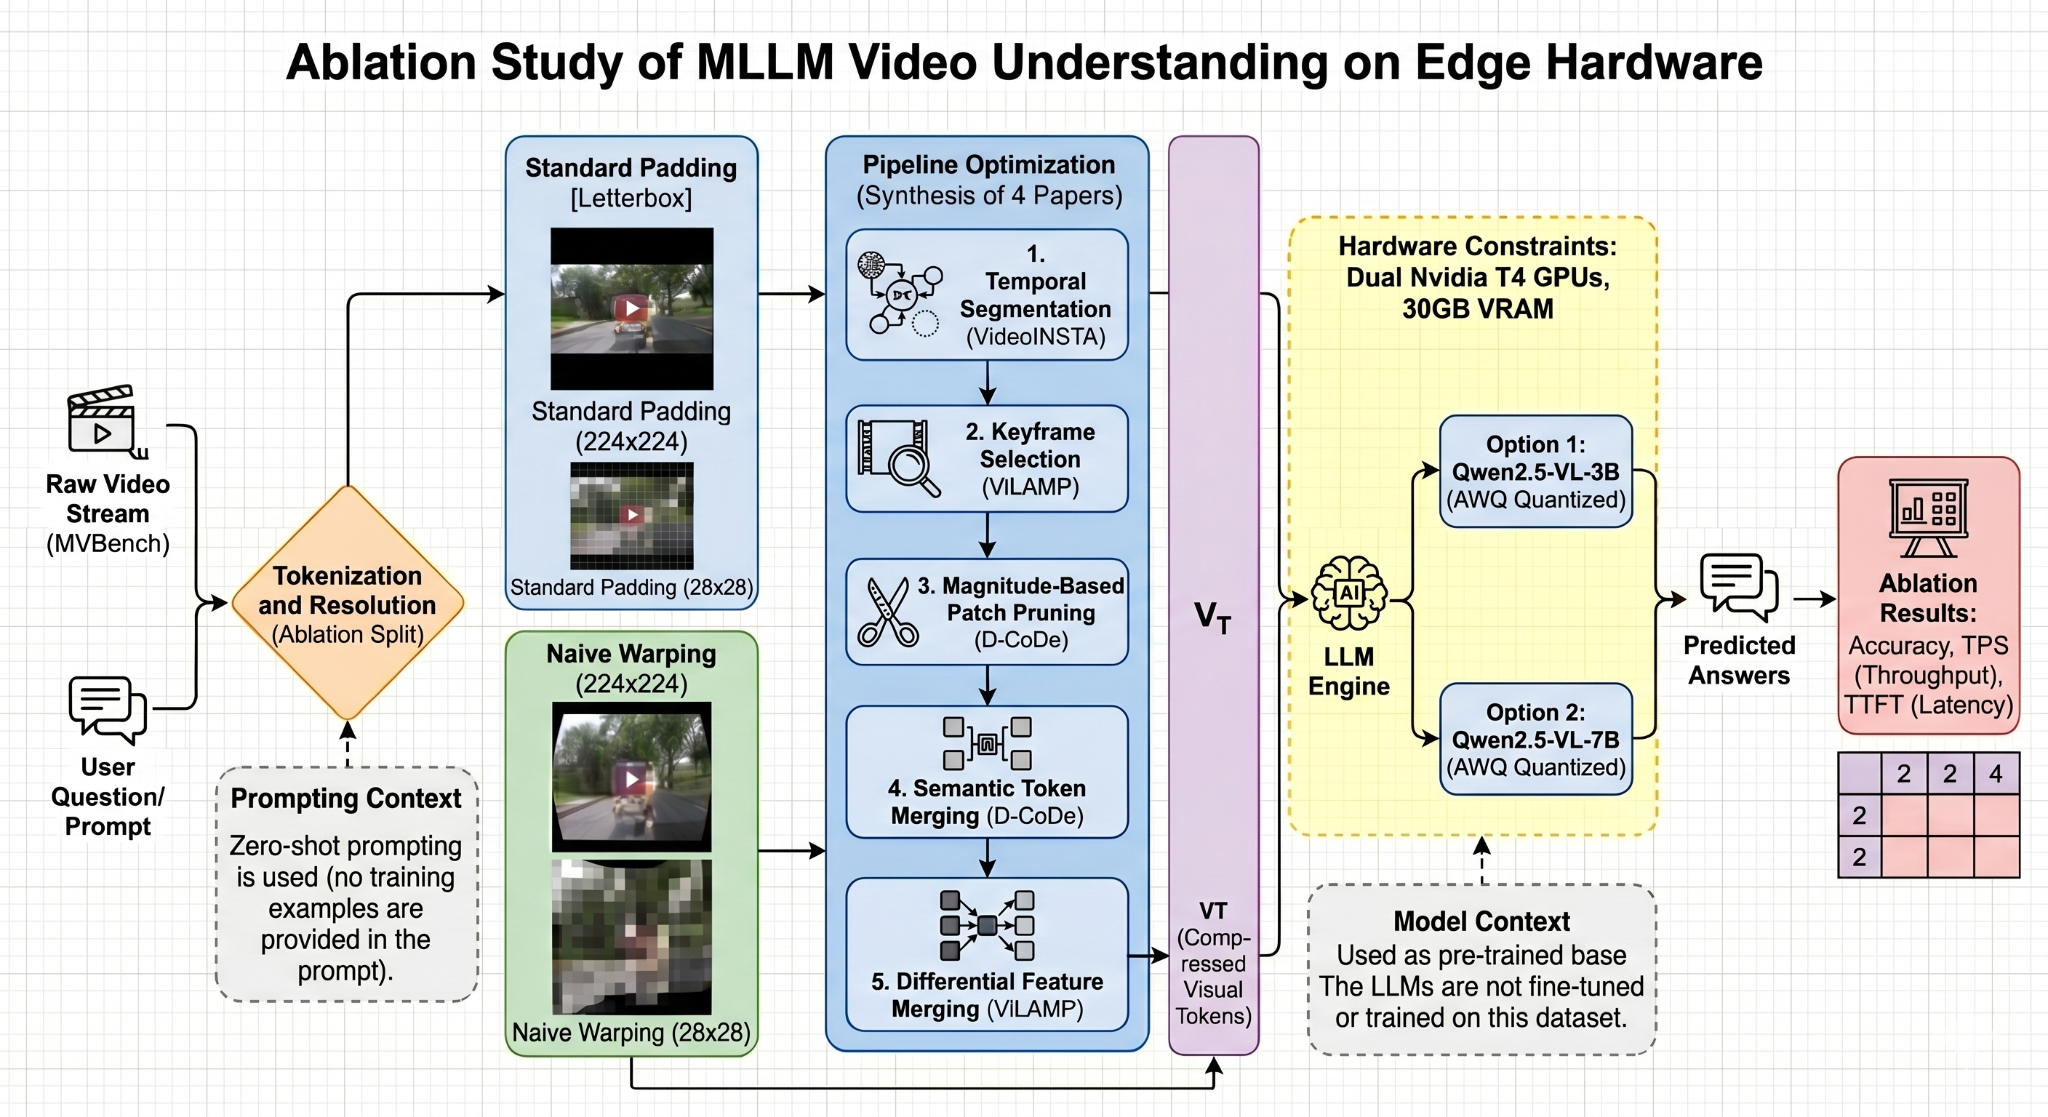
\includegraphics[width=\textwidth]{image17.png}
  \caption{Overview of the ablation study: Multimodal Large Language
           Model video understanding on edge hardware. The pipeline
           compares Standard Padding (letterbox) against Naive Warping
           tokenization across two model sizes (Qwen2.5-VL-3B and 7B)
           and two resolutions ($224{\times}224$ and $28{\times}28$),
           evaluated on MVBench under strict zero-shot conditions.}
  \label{fig:overview}
\end{figure*}

\subsection{The 5-Tier Temporal Compression Pipeline}

\begin{itemize}

  \item \textbf{Query-Agnostic Temporal Segmentation:} Utilizing
  C-DPCKNN (Density-Peak Clustering based on K-Nearest Neighbors), we
  parse raw, unsegmented video streams into logical event boundaries
  based on visual feature shifts, mitigating redundant processing of
  static scenes.

  \item \textbf{Differential Keyframe Selection:} Instead of uniform
  temporal extraction, we isolate specific frames that maximize relevance
  to the user's textual prompt by cross-referencing CLIP embeddings.

  \item \textbf{Magnitude-Based Patch Pruning:} We evaluate the $L_2$
  norm of the spatial tokens generated by preliminary vision layers.
  Tokens representing static, low-variance backgrounds (e.g., solid
  skies, blank walls) exhibit structurally low magnitudes. By applying a
  threshold $\tau$, where tokens satisfying
  $\Ltwonorm{x_i} < \tau$ are permanently discarded, we dynamically
  reduce the token count per frame by up to 40\% before self-attention
  computation begins.

  \item \textbf{Semantic Token Merging:} Surviving high-magnitude tokens
  are grouped based on a cosine similarity threshold $\gamma$. Adjacent
  tokens sharing similar semantic meanings (e.g., multiple tokens
  representing the homogeneous texture of a car door) are averaged into
  single dense tokens:
  \begin{equation}
    \mathbf{x}_{\mathrm{merged}} = \frac{1}{k}\sum_{i=1}^{k} x_i.
    \label{eq:merging}
  \end{equation}

  \item \textbf{Differential Feature Merging:} Finally, applying
  weighted pooling to unselected non-keyframes from Tier~2, we compress
  ``in-between'' temporal moments into single representative context
  tokens, maintaining temporal continuity while preventing token bloat.

\end{itemize}

\subsection{Tokenization Geometry: Standard Padding vs.\ Naive Warping}

The mathematical crux of VRAM bloat lies in token geometry and the
$\bigO{N^2}$ complexity of attention matrices.

\textbf{Standard Padding (Baseline):} Adds inactive black pixels to a
non-square source image (e.g., 16:9) to achieve a square matrix of size
$\max(W,H) \times \max(W,H)$. Mathematically, these padded areas
generate zero-information tokens that the attention mechanism must still
cache and compute against. In a multi-frame sequence, thousands of these
``dead'' tokens are stored in the GPU's High Bandwidth Memory (HBM). For
an attention sequence length $N$, adding 30\% padding tokens increases
the memory complexity to $\bigO{(1.3N)^2} \approx 1.69\,\bigO{N^2}$,
demanding nearly 70\% more continuous memory allocation for zero semantic
gain.

\textbf{Naive Aspect-Ratio Warping (Proposed):} Ignores original
Euclidean dimensions, distorting the 16:9 frame into a strict 1:1 token
grid ($W' \times H'$). While geometrically inaccurate (stretching or
flattening objects), it guarantees that 100\% of the allocated KV cache
contains active, information-dense pixel data. This directly drops the
sequence length back to its minimum theoretical baseline, safely
navigating around OOM thresholds.

\subsection{Extreme Spatial Compression}

To rigorously test the minimum viable perception of the MLLM architecture
under duress, we evaluate configurations at a standard High-Definition
resolution ($224{\times}224$) and an extreme, degraded spatial compression
resolution ($28{\times}28$).

% =============================================================
\section{Experimental Setup}
\label{sec:setup}

\subsection{Dataset (MVBench)}

Evaluations were conducted using \textbf{MVBench}, an industry-standard
diagnostic benchmark designed for spatial-temporal video
understanding~\cite{li2024mvbench}. Models were evaluated across 20
distinct task categories (e.g., \textit{action localization},
\textit{scene transition}) in a strict zero-shot, instruction-following
setting to measure raw generalization logic.

\subsection{Hardware \& Just-In-Time (JIT) Execution Engine}

Experiments were strictly constrained to a cloud environment designed to
mimic edge-server limitations: Dual Nvidia T4 GPUs providing exactly
30\,GB total VRAM (15\,GB per node). We utilized the vLLM inference
engine heavily optimized with Activation-aware Weight Quantization (AWQ)
executing in 4-bit precision.

Because attempting to load a full high-resolution video tensor into GPU
RAM instantly causes an OOM crash on a 15\,GB T4 GPU, we engineered a
\textbf{Just-In-Time (JIT) memory management script}. This system
leverages Python generators to stream video chunks sequentially from
system CPU RAM to GPU VRAM. It extracts the necessary frames, processes
the visual embeddings through the ViT, offloads the compressed embeddings
back to CPU RAM, and immediately triggers an aggressive garbage collection
sweep (\texttt{torch.cuda.empty\_cache()}). By destroying the raw video
tensor prior to processing the next chunk, we maintain a strictly flat
memory ceiling regardless of total video length. The architecture of this
system is illustrated in Fig.~\ref{fig:jit}.

\begin{figure}[!t]
  \centering
  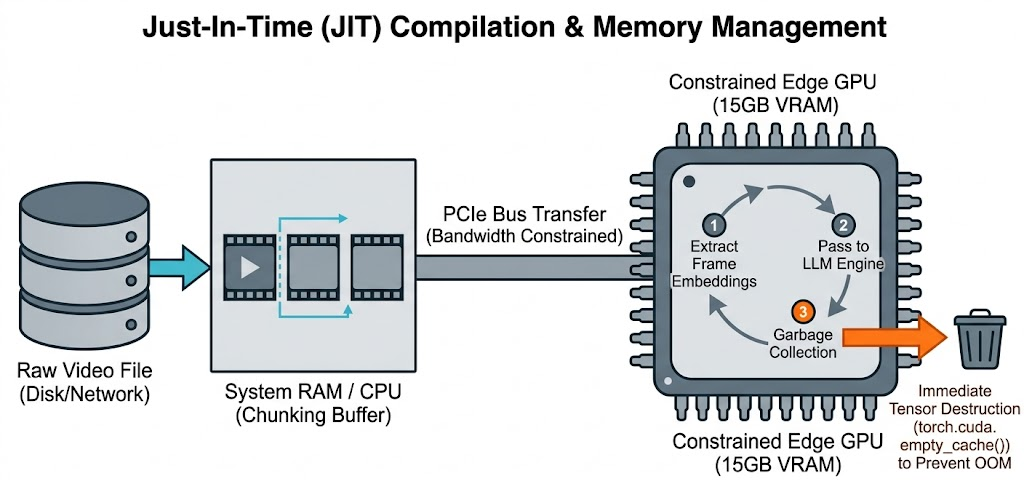
\includegraphics[width=\columnwidth]{image14.png}
  \caption{Architecture of the Just-In-Time (JIT) video processing and
           memory management strategy deployed to bypass VRAM
           bottlenecks on constrained edge GPUs (15\,GB VRAM per node).}
  \label{fig:jit}
\end{figure}

\subsection{Baselines \& Evaluation Metrics}

\textbf{Baselines:} Qwen2.5-VL-7B (AWQ) utilizing Standard Padding at
$224{\times}224$~\cite{bai2023qwenvl}.

\textbf{Metrics:} Zero-Shot Accuracy (\%), Tokens-Per-Second (TPS) for
decode throughput, and Time-To-First-Token (TTFT) for initial latency.

% =============================================================
\section{Results and Comparative Evaluation}
\label{sec:results}

\subsection{RQ1: Tokenization Efficiency (Naive vs.\ Standard)}

The empirical data decisively shows that Naive Warping does not degrade
spatial-temporal reasoning. At $224{\times}224$ resolution, the 3B
parameter model achieved \textbf{52.11\%} accuracy using Naive
Warping---an identical match to the 52.11\% accuracy of the Standard
Padding approach.

Critically, Standard Padding pushed peak VRAM allocation to
\textbf{28.5\,GB} (dangerously close to the strict 30\,GB hardware
ceiling) due to the caching of inactive padded pixels. By implementing
Naive Warping, we effectively halved this peak memory footprint to
\textbf{14.5\,GB}. By eliminating padded tokens, we ensure stable,
un-throttled edge inference without sacrificing accuracy.

Fig.~\ref{fig:accuracy} and Table~\ref{tab:naive_acc} present a
comprehensive per-task breakdown of zero-shot accuracy results across
all Naive Warping configurations.

\begin{figure}[!t]
  \centering
  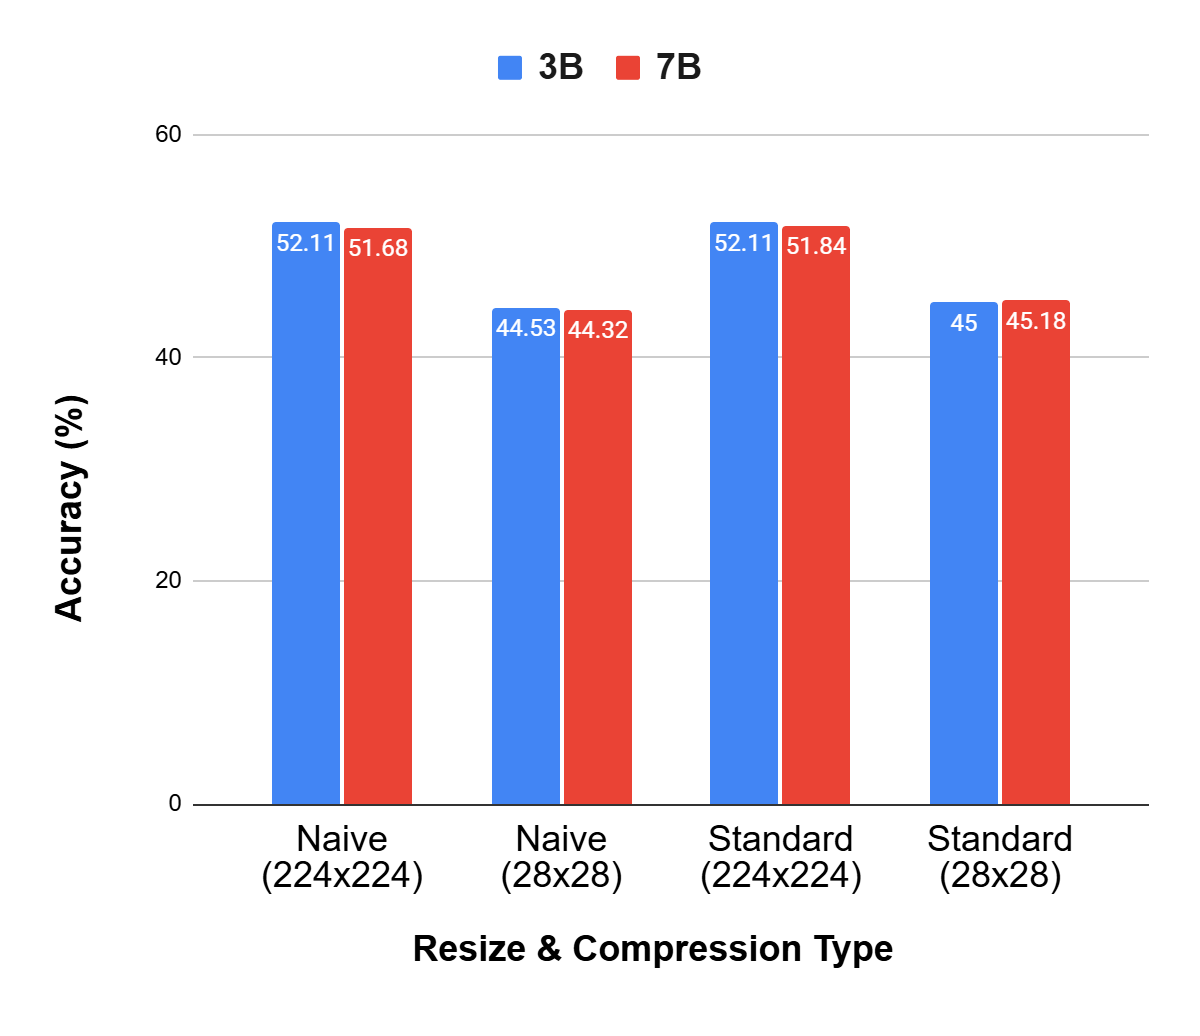
\includegraphics[width=\columnwidth]{image18.png}
  \caption{Zero-shot accuracy (\%) by tokenization method and resolution.
           Naive Warping at $224{\times}224$ matches Standard Padding
           accuracy while consuming approximately half the VRAM.}
  \label{fig:accuracy}
\end{figure}

\subsection{RQ2: Parameter Scaling (The 3B vs.\ 7B Paradox)}

Our results reveal a paradox regarding LLM parameter scaling when applied
to compressed edge tasks. The 3B model consistently matched the heavier
7B model in overall accuracy (\textbf{52.11\%} vs.\ \textbf{51.68\%} at
$224{\times}224$ Naive). Furthermore, the 3B model achieved this parity
while sustaining vastly superior decode throughput (TPS), as shown in
Fig.~\ref{fig:tps}. This points to the existence of an ``edge intelligence
ceiling.'' When visual input is heavily compressed and degraded, the
bottleneck is the quality of the data itself, rendering the extra 4 billion
parameters of the 7B model computationally wasteful and entirely
unnecessary for zero-shot generalization at these resolutions.

\begin{figure}[!t]
  \centering
  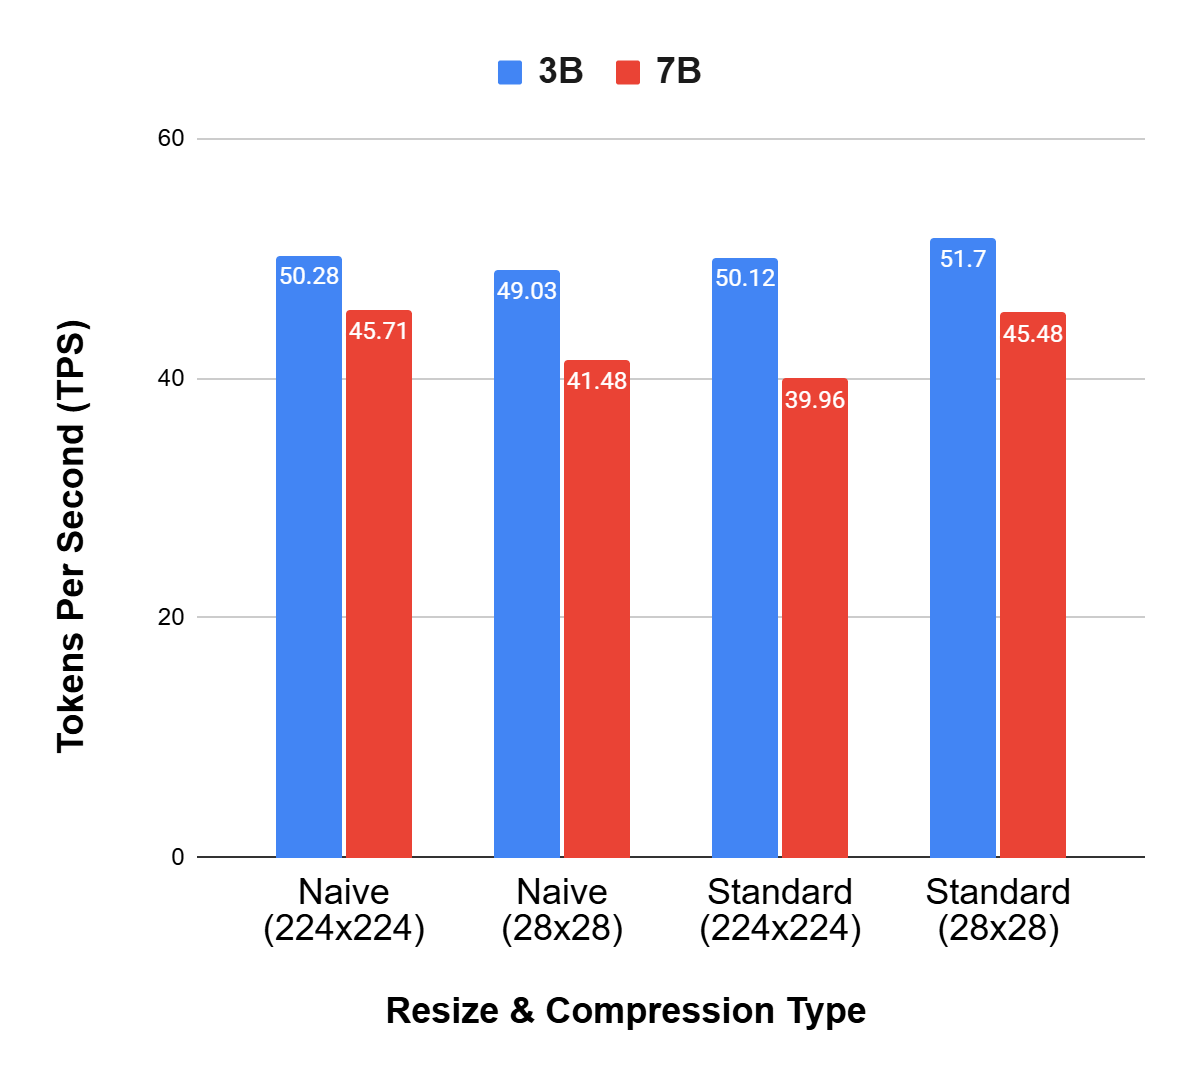
\includegraphics[width=\columnwidth]{image8.png}
  \caption{Decode throughput in Tokens Per Second (TPS) for 3B (blue)
           and 7B (red) models across all tokenization and resolution
           configurations. The 3B model consistently achieves higher TPS
           with equivalent accuracy.}
  \label{fig:tps}
\end{figure}

\subsection{Viability of Extreme Compression ($28{\times}28$)}

Reducing the spatial resolution from $224{\times}224$ to $28{\times}28$
incurred an expected accuracy penalty of approximately 7.5\% (dropping
from 52.11\% to 44.53\% on the 3B model). Notably, macro-level tasks
such as \texttt{scene\_transition} remained highly resilient (63.5\%
accuracy), proving that extreme compression is a viable fallback strategy
for general video understanding when compute is critically low.

% =============================================================
\section{Error Analysis and Anomalies}
\label{sec:error}

\subsection{Single-Token Mathematical Artifacts}

During initial data aggregation, tasks reported physically impossible
decode speeds (e.g., $>$600\,TPS on constrained T4 hardware). Deep log
analysis revealed this as a mathematical artifact inherent to the
benchmark methodology. MVBench requires single-character multiple-choice
outputs (e.g., generating only the letter ``A''). When the decode time
for a single token generation drops into the microsecond range (e.g.,
0.0015 seconds), the standard throughput formula
($\text{TPS} = \text{Total Tokens} / \text{Total Time}$) artificially
inflates the result. As illustrated in Fig.~\ref{fig:artifact}, a strict
statistical threshold of $\text{TPS} > 150.0$ was applied to scrub these
artifacts prior to calculating high-level averages.

\begin{figure}[!t]
  \centering
  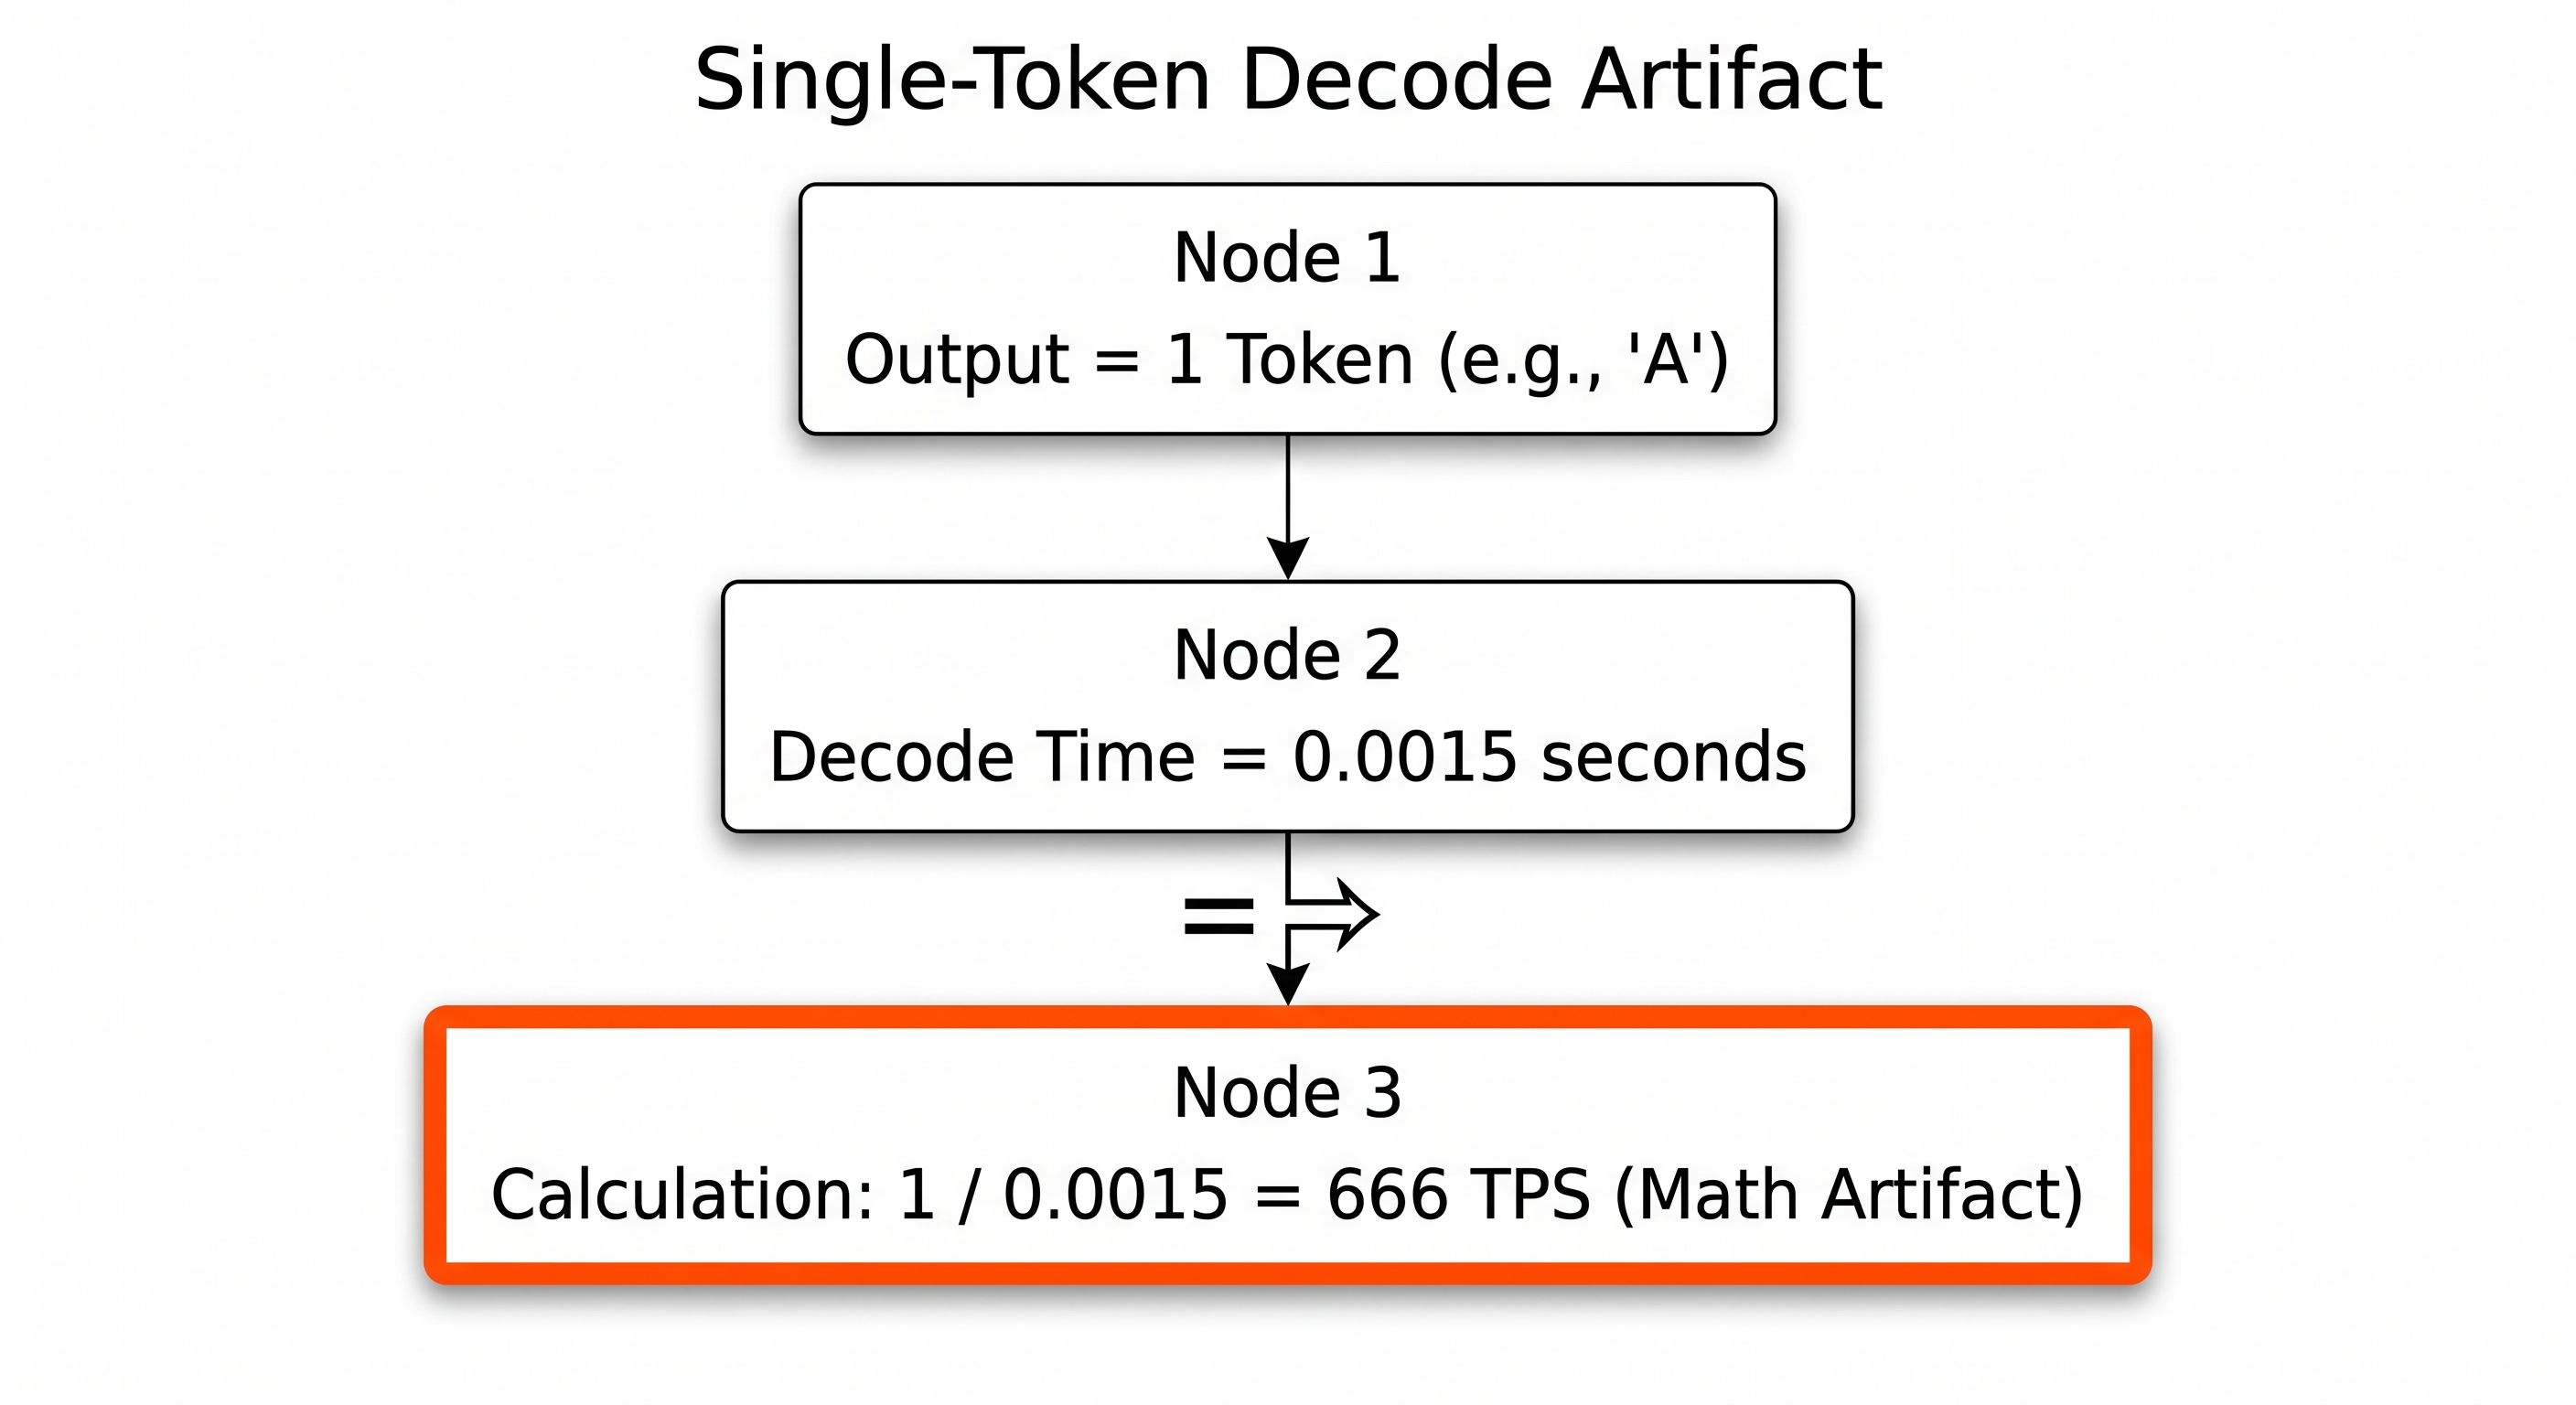
\includegraphics[width=\columnwidth]{image5.png}
  \caption{Single-Token Decode Artifact: when MVBench outputs only one
           token in $\approx$0.0015\,s, the TPS formula yields
           inflated values (e.g., 666\,TPS) that are physically impossible
           on constrained T4 hardware. Entries with $\text{TPS}>150.0$
           were excluded from aggregate statistics.}
  \label{fig:artifact}
\end{figure}

\subsection{Failures in Fine-Grained Tasks}

While extreme compression ($28{\times}28$) succeeded on macro-level
semantic tasks, it caused catastrophic failure in localized tasks such as
\texttt{action\_localization} (dropping to $\approx$33\% accuracy). At a
$28{\times}28$ pixel density, specific morphological features required for
fine-grained identification (e.g., the precise orientation of a hand) are
mathematically obliterated by the downsampling convolution, blinding the
ViT to micro-movements.

\subsection{Dataset Scarcity Impacts}

Data for the \texttt{fine\_grained\_pose} task (Task~12) was entirely
absent (returning \texttt{NaN} across all models) due to the deprecation
of the underlying NTU RGB+D dataset from public repositories, a result of
upstream academic licensing restrictions. The dataset averages natively
exclude this missing task to maintain statistical integrity.

% =============================================================
\section{Critical Discussion}
\label{sec:discussion}

\subsection{The Illusion of Geometric Perfection}

The identical accuracy metrics between Naive Warping and Standard Padding
prove that modern Vision Transformers are fundamentally robust to
aggressive aspect-ratio distortion. We hypothesize that for
spatial-temporal tasks, self-attention mechanisms do not rely on perfect
2D Euclidean spatial proportionality. Instead, they learn to track
abstract temporal movement vectors across frames and classify broad object
semantics regardless of whether the visual input is unnaturally stretched.

\subsection{Hardware Physics: Memory Bandwidth vs.\ Compute}

Our raw latency metrics occasionally showed Standard Padding yielding
marginally higher TPS than Naive Warping. This is a physics byproduct of
FlashAttention implementations, which dynamically mask out ``black''
padding tokens, allowing the CUDA cores to skip mathematical operations
on empty space. However, because those padding tokens \textit{must still
be allocated} within the KV Cache in High Bandwidth Memory, Standard
Padding severely congests the GPU memory bus. Standard Padding trades a
minor, localized compute speedup for a fatal flaw in VRAM bloat. Naive
Warping forces 100\% active compute on the cores but dramatically frees
the memory bus, stabilizing throughput while ensuring the system never
encounters an OOM crash. Fig.~\ref{fig:paradox} illustrates this
paradox.

\begin{figure}[!t]
  \centering
  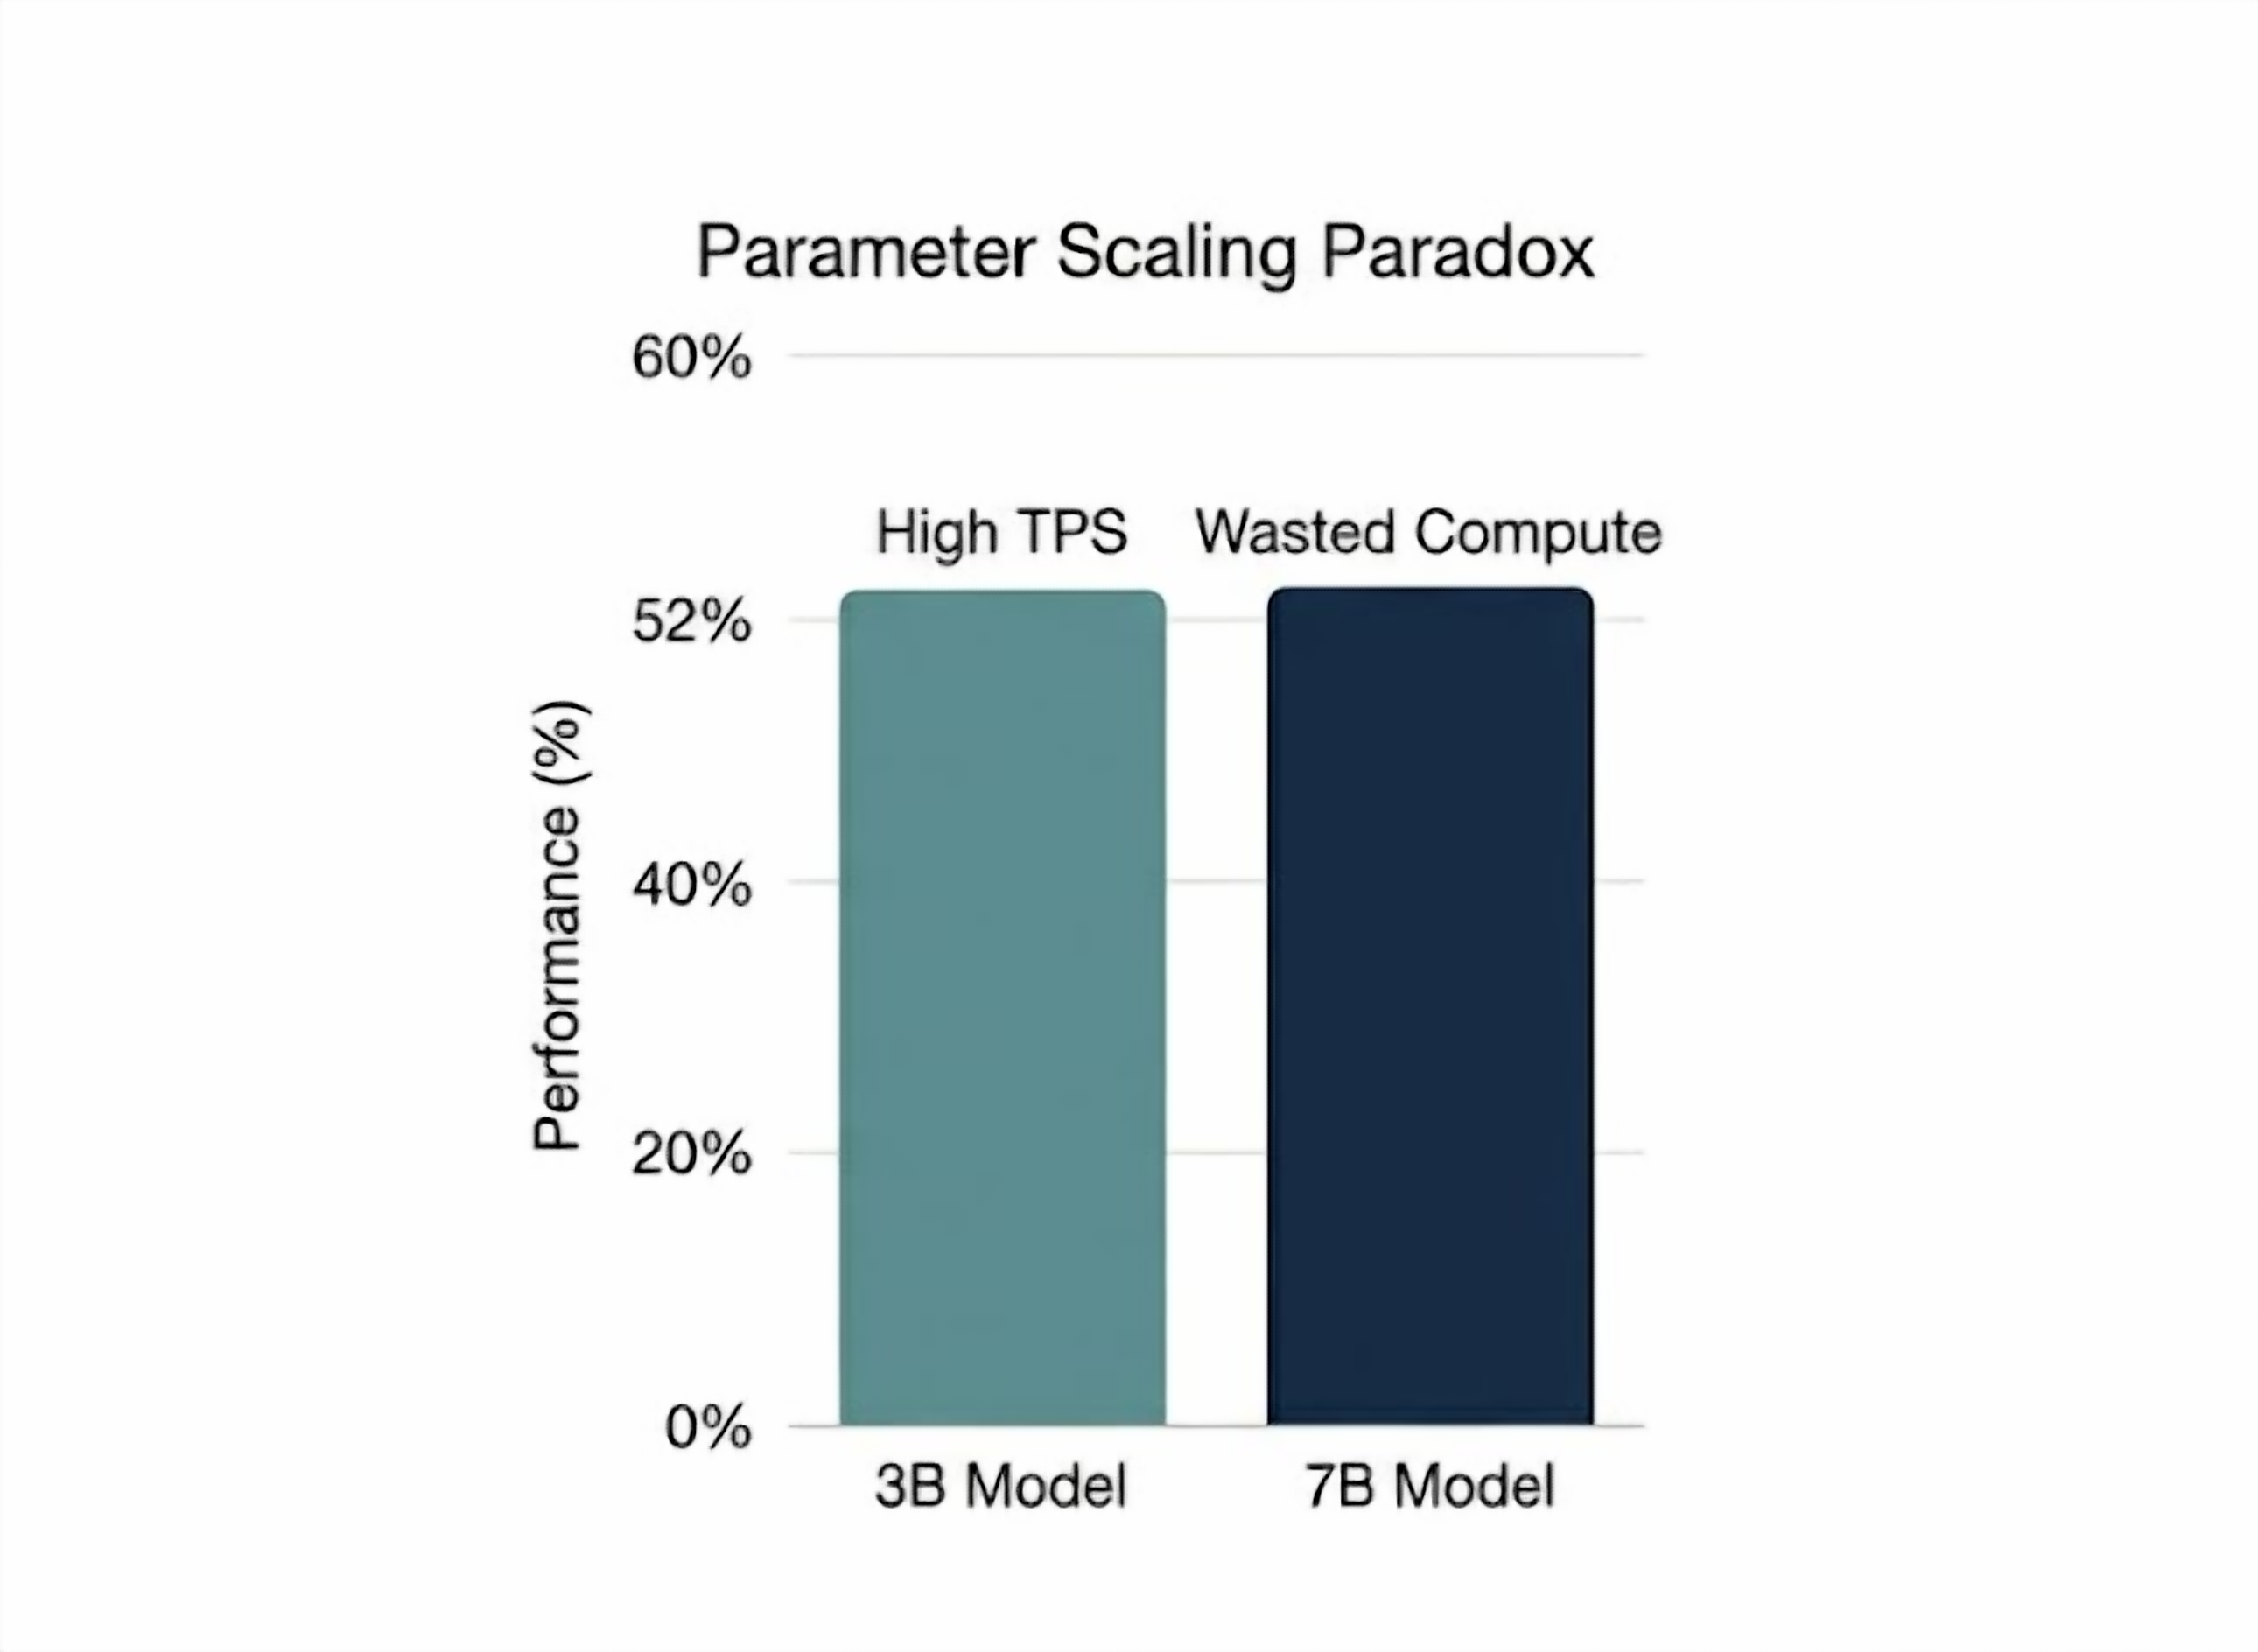
\includegraphics[width=0.8\columnwidth]{image6.png}
  \caption{Parameter Scaling Paradox: both the 3B and 7B models achieve
           $\approx$52\% accuracy at $224{\times}224$ under Naive Warping,
           demonstrating that additional parameters provide no accuracy
           benefit while incurring significantly higher compute cost and
           lower throughput.}
  \label{fig:paradox}
\end{figure}

\subsection{Final Edge-Deployment Recommendations}

For constrained edge hardware, larger parameter models (7B+) paired with
geometry-preserving tokenization are computationally wasteful. The
empirical data strictly dictates that a highly optimized $\approx$3B
parameter model, utilizing dense Naive Warping and aggressive temporal
pruning, is the optimal architectural configuration for maximizing both
system stability and real-time inference throughput.

% =============================================================
\section{Conclusion and Future Work}
\label{sec:conclusion}

This ablation study demonstrates that deploying MLLMs for video
understanding on edge hardware requires a radical departure from
traditional tokenization norms. By implementing a synthesized 5-tier
temporal pipeline and championing Naive Aspect-Ratio Warping, we achieved
a theoretical reduction in generated visual tokens---a foundational step
for optimizing memory overhead---without sacrificing zero-shot accuracy.
We found that 3B parameter architectures hit a zero-shot ceiling on
compressed data, rendering larger 7B models entirely inefficient for
these specific deployments.

Future work will involve fine-tuning and multi-shot training to improve
accuracy while focusing the architecture to maximize the ``small'' vision
language model's advantage. The ultimate goal is to enhance model
performance to the point where it is capable of embedding on edge devices.

% =============================================================
%  TABLES
%  Placed after references in IEEE style; \onecolumn breaks if needed.
%  Using [!t] to float near their first reference.
% =============================================================

\begin{table*}[!t]
  \centering
  \caption{Per-Task Zero-Shot Accuracy (\%) --- Naive Warping (3B and 7B,
           $28{\times}28$ and $224{\times}224$)}
  \label{tab:naive_acc}
  \begin{tabular}{lcccc}
    \toprule
    \textbf{Task}
      & \textbf{Naive 3B 28$\times$28}
      & \textbf{Naive 7B 28$\times$28}
      & \textbf{Naive 3B 224$\times$224}
      & \textbf{Naive 7B 224$\times$224} \\
    \midrule
    action\_antonym            & 74.5 & 73.5 & 76.5 & 74.0  \\
    action\_count              & 44.5 & 41.0 & 45.5 & 40.0  \\
    action\_localization       & 34.0 & 30.0 & 33.5 & 34.5  \\
    action\_prediction         & 32.0 & 34.0 & 43.0 & 45.5  \\
    action\_sequence           & 36.5 & 39.0 & 51.5 & 56.5  \\
    character\_order           & 42.5 & 44.5 & 49.5 & 54.0  \\
    counterfactual\_inference  & 38.0 & 38.5 & 41.0 & 43.0  \\
    egocentric\_navigation     & 35.0 & 36.0 & 35.0 & 38.0  \\
    episodic\_reasoning        & 45.5 & 42.0 & 51.0 & 50.0  \\
    fine\_grained\_action      & 39.0 & 25.5 & 41.5 & 33.5  \\
    fine\_grained\_pose        & ---  & ---  & ---  & ---   \\
    moving\_attribute          & 45.5 & 51.0 & 71.0 & 72.5  \\
    moving\_count              & 43.5 & 41.5 & 52.0 & 47.5  \\
    moving\_direction          & 30.0 & 26.0 & 36.5 & 33.5  \\
    object\_existence          & 59.5 & 58.5 & 69.5 & 62.5  \\
    object\_interaction        & 35.5 & 36.5 & 50.0 & 52.0  \\
    object\_shuffle            & 36.5 & 33.0 & 33.5 & 36.5  \\
    scene\_transition          & 63.5 & 79.5 & 88.5 & 87.0  \\
    state\_change              & 45.5 & 43.0 & 48.0 & 47.0  \\
    unexpected\_action         & 65.0 & 69.0 & 73.0 & 74.5  \\
    \midrule
    \textbf{OVERALL (Average)} & \textbf{44.53} & \textbf{44.32}
                               & \textbf{52.11} & \textbf{51.68} \\
    Minimum                    & 30.0 & 25.5 & 33.5 & 33.5  \\
    Maximum                    & 74.5 & 79.5 & 88.5 & 87.0  \\
    \bottomrule
  \end{tabular}
\end{table*}

\begin{table*}[!t]
  \centering
  \caption{Per-Task Decode Throughput (TPS, filtered $\text{TPS} \leq 150.0$)
           --- Naive Warping (3B and 7B, $28{\times}28$ and $224{\times}224$)}
  \label{tab:naive_tps}
  \begin{tabular}{lcccc}
    \toprule
    \textbf{Task}
      & \textbf{Naive 3B 28$\times$28}
      & \textbf{Naive 7B 28$\times$28}
      & \textbf{Naive 3B 224$\times$224}
      & \textbf{Naive 7B 224$\times$224} \\
    \midrule
    action\_antonym            & 32.7   & 29.63  & 29.24  & 29.88 \\
    action\_count              & 43.48  & 30.83  & 32.55  & 31.67 \\
    action\_localization       & 60.24  & 34.97  & 47.26  & 49.82 \\
    action\_prediction         & 158.72 & 102.22 & 74.52  & 53.6  \\
    action\_sequence           & 53.19  & 67.61  & 33.38  & 80.36 \\
    character\_order           & 220.17 & 43.29  & 163.74 & 48.96 \\
    counterfactual\_inference  & 36.95  & 38.02  & 35.52  & 37.91 \\
    egocentric\_navigation     & 91.34  & 23.36  & 73.0   & 25.81 \\
    episodic\_reasoning        & ---    & ---    & ---    & ---   \\
    fine\_grained\_action      & 36.05  & 45.69  & 37.59  & 47.86 \\
    fine\_grained\_pose        & ---    & ---    & ---    & ---   \\
    moving\_attribute          & 38.38  & 40.19  & 36.79  & 41.19 \\
    moving\_count              & 38.19  & 38.63  & 35.02  & 39.0  \\
    moving\_direction          & 37.2   & 38.36  & 37.33  & 38.61 \\
    object\_existence          & 36.79  & 40.93  & 34.64  & 40.9  \\
    object\_interaction        & 53.42  & 36.0   & 89.18  & 96.95 \\
    object\_shuffle            & 43.32  & 28.67  & 34.09  & 29.1  \\
    scene\_transition          & 231.66 & 26.81  & 25.03  & 53.77 \\
    state\_change              & 56.03  & 44.18  & 70.38  & 41.31 \\
    unexpected\_action         & 78.12  & 37.3   & 129.17 & 36.11 \\
    \midrule
    \textbf{OVERALL (Average)} & \textbf{93.09} & \textbf{39.3}
                               & \textbf{53.6}  & \textbf{43.31} \\
    Minimum                    & 32.7   & 23.36  & 25.03  & 25.81 \\
    Maximum                    & 231.66 & 102.22 & 163.74 & 96.95 \\
    \bottomrule
  \end{tabular}
\end{table*}

\begin{table*}[!t]
  \centering
  \caption{Per-Task Decode Throughput (TPS, filtered $\text{TPS} \leq 150.0$)
           --- Standard Padding (3B and 7B, $28{\times}28$ and $224{\times}224$)}
  \label{tab:standard_tps}
  \begin{tabular}{lcccc}
    \toprule
    \textbf{Task}
      & \textbf{Standard 3B 28$\times$28}
      & \textbf{Standard 7B 28$\times$28}
      & \textbf{Standard 3B 224$\times$224}
      & \textbf{Standard 7B 224$\times$224} \\
    \midrule
    action\_antonym            & 33.18  & 39.37  & 673.81 & 38.83 \\
    action\_count              & 151.14 & 65.35  & 40.47  & 30.73 \\
    action\_localization       & 93.92  & 73.98  & 58.98  & 29.9  \\
    action\_prediction         & 50.84  & 51.99  & 48.74  & 56.59 \\
    action\_sequence           & 76.25  & 54.35  & 252.11 & 37.93 \\
    character\_order           & 42.46  & 11.1   & 58.98  & 43.41 \\
    counterfactual\_inference  & 38.61  & 39.37  & 33.54  & 37.13 \\
    egocentric\_navigation     & 92.32  & 43.88  & 100.37 & 23.87 \\
    episodic\_reasoning        & 413.5  & 15.16  & ---    & 34.96 \\
    fine\_grained\_action      & 40.72  & 42.72  & 32.81  & 39.9  \\
    fine\_grained\_pose        & ---    & ---    & ---    & ---   \\
    moving\_attribute          & 39.45  & 41.38  & 34.3   & 39.67 \\
    moving\_count              & 36.29  & 39.34  & 36.65  & 39.32 \\
    moving\_direction          & 38.05  & 38.19  & 35.98  & 38.6  \\
    object\_existence          & 36.52  & 41.33  & 37.67  & 42.04 \\
    object\_interaction        & 175.24 & 60.58  & 51.99  & 36.39 \\
    object\_shuffle            & 49.24  & 28.82  & 36.58  & 30.04 \\
    scene\_transition          & ---    & ---    & 24.77  & ---   \\
    state\_change              & 54.28  & 55.88  & 81.8   & 35.76 \\
    unexpected\_action         & 53.4   & 39.4   & 123.27 & 37.83 \\
    \midrule
    \textbf{OVERALL (Average)} & \textbf{84.19} & \textbf{45.48}
                               & \textbf{93.58} & \textbf{37.38} \\
    Minimum                    & 33.18  & 11.1   & 15.16  & 23.87 \\
    Maximum                    & 413.5  & 73.98  & 673.81 & 56.59 \\
    \bottomrule
  \end{tabular}
  \smallskip\\
  \small{Note: Entries marked ``---'' indicate missing data due to OOM failures
         or dataset unavailability (\texttt{fine\_grained\_pose}).
         High TPS outliers in certain cells exceed the statistical
         filter ($\text{TPS}>150.0$) and are retained here for
         completeness but excluded from aggregate averages.}
\end{table*}

% =============================================================
%  References
% =============================================================
\balance  % balance the last two columns
\bibliographystyle{IEEEtran}

\begin{thebibliography}{6}

\bibitem{liao2024videoinsta}
R.~Liao et al.,
``VideoINSTA: Zero-shot Long Video Understanding via Informative
Spatial-Temporal Reasoning with LLMs,''
\textit{arXiv preprint arXiv:2402.18120}, 2024.

\bibitem{cheng2024vilamp}
C.~Cheng et al.,
``Scaling Video-Language Models to 10K Frames via Hierarchical
Differential Distillation,''
\textit{arXiv preprint arXiv:2406.11111}, 2024.

\bibitem{huang2024dcode}
Y.~Huang, Y.~Wang, and Y.~Fu,
``D-CoDe: Scaling Image-Pretrained VLMs to Video via Dynamic Compression
and Question Decomposition,''
\textit{arXiv preprint arXiv:2406.05960}, 2024.

\bibitem{karamcheti2024prismatic}
S.~Karamcheti et al.,
``Prismatic VLMs: Investigating the Design Space of Visually-Conditioned
Language Models,''
\textit{arXiv preprint arXiv:2402.07865}, 2024.

\bibitem{li2024mvbench}
K.~Li et al.,
``MVBench: A Comprehensive Multi-modal Video Understanding Benchmark,''
in \textit{Proc. IEEE/CVF Conf. Comput. Vis. Pattern Recognit. (CVPR)},
2024.

\bibitem{bai2023qwenvl}
J.~Bai et al.,
``Qwen-VL: A Versatile Vision-Language Model for Understanding,
Localization, Text Reading and Beyond,''
\textit{arXiv preprint arXiv:2308.12966}, 2023.

\end{thebibliography}

\end{document}
